\section{Principal Component Analysis(PCA)}
	Sometimes, the dimension of input data is very large, we need to reduce the dimension before analyzing it. The \textbf{Principal Component Analysis} is a popular method of dimensional reduction.
	
	Suppose $\mathbf x_1,...,\mathbf x_n\in\mathbb R^d$ are the input data ($d\gg 1$), and satisfy $\sum_{i=1}^{n}\mathbf x_i=\mathbf 0$. Write $\mathbf X = (\mathbf x_1,...,\mathbf x_n)$. We want to find a subspace $\mathbb F$ (dim$\mathbb F$ = k) of $\mathbb{R}^d$ such that each projections of $\mathbf x_i$ in $\mathbb F$ is as close as possible to $\mathbf x_i$. The effect of PCA on MNist Dataset is showed in Figure \ref{fig:mnistpca}.
	
	\begin{figure}[h]
		\centering
		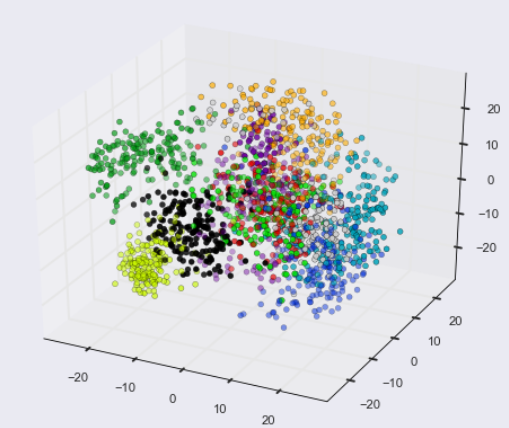
\includegraphics[width=0.7\linewidth]{MNistPCA}
		\caption{The effect of PCA on MNist Dataset, where $\dim \mathbb F=3$}
		\label{fig:mnistpca}
	\end{figure}

\subsection{The Case of k=1: The First Component}


	In the 1-d case, the subspace $\mathbb F$ is a line which goes through the original point in $\mathbb R^d$, let's write the direction vector of $\mathbb F$ as $\mathbf w$, where $\|\mathbf w\|_2=1$. Then $\mathbb F=\text{span}\{\mathbf w\}$ $\sum_{i=1}^N x_i=0$. The projections of $\mathbf x_1,...,\mathbf x_n$ in $\mathbb F$ is $\mathbf y_1,...,\mathbf y_n$, i.e.
	\begin{align}
	y_i&=\alpha_i \mathbf w \\\notag
	(y_i,\mathbf w)&=(x_i ,\mathbf w) \\\notag
	\alpha_i &=(x_i ,\mathbf w)=\mathbf w^T\mathbf x_i \\\notag
	\end{align}

	 $$\mathbf y_i=(\mathbf w^T\mathbf x_i)\mathbf w=\mathbf w \mathbf w^T\mathbf x_i.$$
	  So we can easily get 
	$$\sum_{i=1}^{n}\mathbf y_i=\sum_{i=1}^{n}(\mathbf w^T\mathbf x_i)\mathbf w=\sum_{i=1}^{n}\mathbf w^T(\sum_{i=1}^{n}\mathbf x_i)\mathbf w=\bm 0.$$

\begin{itemize}
\item Maximize the Variance (from the point of statistical learning)	

	Because the more point $\mathbf y_1,...,\mathbf y_n$ is decentralized, the easily we classify them. And we can use the variance to measure the degree of decentralization of these points. So our goal is to find the line, maximizes the variance of  $\mathbf y_1,...,\mathbf y_n$, i.e.

	\begin{align*}
	\max_{\|\mathbf w\|^2_2=1}f(\textbf w)
	&=Var(\textbf y) = \sum_i \mathbf ||\mathbf y_i-\dfrac{1}{n}\sum_{i=1}^{n}\mathbf y_i||_2^2\\
	&= \sum_i \mathbf ||\mathbf y_i-\mathbf 0||_2^2= \sum_i(\textbf w^T \textbf x_i)^2 \hspace{1cm} (\text{use} \|\mathbf w\|_2=1)
	\end{align*}

\item Minimize distance (form the point of autoencoder)

	In other opinion, we want the distance between $\mathbf x_i$ and $\mathbf y_i$ can be as small as possible. So we can minimize 
	\begin{align*}
	\min_{\|\mathbf w\|^2_2=1}g(\textbf w)
	=&\sum_i \mathbf ||\mathbf y_i-\mathbf x_i||_2^2\\
	=&\sum_i \mathbf( ||\mathbf y_i||_2^2-2\mathbf x_i^T\mathbf y_i + ||\mathbf x_i||_2^2)\\
	=&-\sum_i(\textbf w^T \textbf x_i)^2+\sum_i||\mathbf x_i||_2^2
	\end{align*}
	So our goal is to find the optimal $\mathbf w$ 
	\begin{align}
	\mathbf w&=\arg\max_{||\mathbf w||^2=1} f(\mathbf w)=\arg\max_{||w||^2=1} \sum_i(\textbf w^T \textbf x_i)^2 \\\notag
	&= \arg\max_{||\mathbf w||^2=1} \sum_i\textbf w^T \textbf x_i \textbf x_i^T  \sum_i\textbf w 
	= \arg\max_{||\mathbf w||^2=1} \textbf w^T XX^T  \sum_i\textbf w   \hspace{1cm}
	\end{align}

\item Solve this problem:

	Its Lagrange multiplier: $$L(\textbf w,\mu )=\sum_i(\textbf w^T \textbf x_i)^2-\mu(\textbf w^T \textbf w-1),$$
	Then we get gradient of $L$:
	$$\nabla_{\mathbf w} L=2(\sum_i \textbf x_i \textbf x_i^T)\mathbf w-2\mu  \mathbf w=0,$$
	$$\nabla_{\mu} L=\mathbf w^T \mathbf w-1=0,$$
	and we can obtain $$S\mathbf w=(\sum_i \textbf x_i \textbf x_i^T)\textbf w=\mu \mathbf w,$$
	where $\textbf S=\sum_i \textbf x_i \textbf x_i^T=\mathbf X\mathbf X^T \in \mathbb{R}^{d\times d}$.v Then $\mu$ and $\textbf w$ is the eigenvalue and corresponding eigenvector of $\mathbf S$. It is easy to calculator that
	 $$f(\mathbf w)=\mathbf w^T \mathbf S \mathbf w =\mu \mathbf w^T\mathbf w =\mu.$$
\end{itemize}	 
	 So we can get a theorem:
	\begin{theorem}\label{PCA}  $\mathbf w$ is the corresponding eigenvector of the max eigenvalue of $\mathbf S=\mathbf X\mathbf X^T$.
	\end{theorem}
	
	Besides, we call $\mathbf x_i\cdot \mathbf w$ the first component of data $\mathbf X$, and $\mathbf w$ is the first component vector.

\subsection{The Case of High Dimensions: Further Components}
	Suppose $\dim \mathbb F = k$, and we have calculated the first component, then we reduce the first component: $\hat{\mathbf X}=\mathbf X - \mathbf w\mathbf w^T\mathbf X$. Now we use  $\mathbf w_{2}^T\mathbf x = \bm 0$ to represent $\mathbb F_2$ and do the same work as the 1-d case.
	By \textbf{theorem} \ref{PCA} we can get $\mathbf w_2$ is the corresponding eigenvector of the max eigenvalue of $\hat{\mathbf S}=\hat{\mathbf X}\hat{\mathbf X}^T$.
	
	Let $\mathbf X = \mathbf U \bm \Sigma \mathbf V^T$ is the SVD decomposition of $\mathbf X$, where $\mathbf U=(\mathbf u_1,...,\mathbf u_n), \bm \Sigma = \text{diag}(\sigma_1,...,\sigma_n)$, $\mathbf  V=(\mathbf v_1,...,\mathbf v_n)$. We have
	$$\mathbf S = \mathbf U \bm \Sigma^2\mathbf U^T,$$ so $\mathbf w =\mathbf u_1$, and
	
	 \begin{align*}\hat{\mathbf X} =& \mathbf X - \mathbf w\mathbf w^T\mathbf X\\
	 =&\mathbf U \bm \Sigma \mathbf V^T-\sigma_1 \mathbf u_1\mathbf v_1^T\\
	 =&\sum_{i=1}^n \sigma_i \mathbf u_i\mathbf v_i^T-\sigma_1 \mathbf u_1\mathbf v_1^T\\
	 =&\sum_{i=2}^n \sigma_i \mathbf u_i\mathbf v_i^T\\
	 =&(\bm 0,\mathbf u_2,...,\mathbf u_n)\text{diag} (0,\sigma_2,...,\sigma_n)(\bm 0,\mathbf v_2,...,\mathbf v_n)^T
	 \end{align*}
	 
	 So the corresponding eigenvector of the max eigenvalue of $\hat{\mathbf S}$ is the corresponding eigenvector of the second big eigenvalue of $\mathbf S$. If we generalize this conclusion, we can get the theorem:
	\begin{theorem} 
	 	The $i$-th component vector $\mathbf w_i$ is the corresponding eigenvector of the $i$-th big eigenvalue of $\mathbf S=\mathbf X\mathbf X^T$, i.e. the $i$-th big left singular value of $\mathbf S=\mathbf X$.
	\end{theorem}
	\begin{remark}
	Suppose the eigenvalues are listed in a descending order as $$\mu_1\geq \mu_2\geq ...\geq...$$ Take $\sigma_i=\sqrt{\mu_i}$, then $\sigma$s are called the corresponding  singular values.
	\end{remark}


\subsection{A General Proof}
	Suppose $\text{dim}\mathbb F = k$,  $\mathbf{W}=(\mathbf{w}_1,...,\mathbf{w}_k)$, and $\mathbb F=\text{span}\{\mathbf{w}_1,...,\mathbf{w}_k\}$ ($\mathbf{w}_j^T\mathbf{w}_j=1,\mathbf{w}_i^T\mathbf{w}_j=0, i\neq j$), then the projection of $\mathbf x_i$ is
	\begin{equation}
		\mathbf{y}_i=\sum_{j=1}^{k}(\mathbf{w}_j^T \mathbf{x}_i)\mathbf{w}_j=\mathbf W\mathbf W^T\mathbf x_i=\mathbf W \tilde{\mathbf x}_i.
	\end{equation}
	
	By the previous discussion, our goal is also to maximize the variance of $\mathbf y_i$, $i=1,...,n$.
	
	Because
	\begin{align*}
	f(\textbf W)
	&=Var(\textbf y) = \sum_i \mathbf ||\mathbf y_i-\dfrac{1}{n}\sum_{i=1}^{n}\mathbf y_i||_2^2\\
	&= \sum_i \mathbf ||\mathbf y_i-\mathbf 0||_2^2\\
	&= \sum_i\sum_j^k(\textbf w_j^T \textbf x_i)^2 \hspace{1cm} (\text{use} \|\mathbf w_j\|_2=1)\\
	&=\sum_j^k\textbf w_j^T \mathbf{S} \textbf w_j, \\
	\end{align*}
	since $w_i^T w_j=\delta_{ij}$, we get a optimal problem:
	
	\begin{equation}
	\max_{\mathbf W^T\mathbf W=\mathbf I}f(\mathbf W)=\sum_j^k\textbf w_j^T \mathbf{S} \textbf w_j= \text{tr}(\mathbf W^T\mathbf S\mathbf W)
	\end{equation}
	The Lagrange multiplier of $f(\mathbf W)$ is: 
	\begin{equation}
	L(\textbf W,\bm \mu)
	=\sum_j\textbf w_j^T \mathbf{S} \textbf w_j-\sum_j\mu_{jj}(\textbf w_j^T \textbf w_j-1)-2\sum_{j< s} \mu_{js}(\textbf w_j^T \textbf w_s-0)
	\end{equation}
	The derivative of $L$ is
	\begin{equation}
	0=\dfrac{\partial L}{\partial \mathbf w_j}=2(\mathbf{S}\mathbf w_j-\sum_s \mu_{js}  \mathbf w_s), \hspace{1cm} \mu_{js}=\mu_{sj}
	\end{equation}
	the we have
	\begin{equation}
	\mathbf{S}\mathbf w_j=\sum_s \mu_{js}  \mathbf w_s,\hspace{1cm} j=1,2,...,k.
	\end{equation}
	
	So the subspace $\mathbb F=\text{span}\{\mathbf w_1,...,\mathbf w_k \} $ is the invariant subspace of $\mathbf S$, then we can obtain that there are $k$ unit eigenvectors $\mathbf u_1,...,\mathbf u_k$ of $\mathbf S$ s.t. $\text{span}\{\mathbf u_1,...,\mathbf u_k \}=\mathbb F$.
	Let $\lambda_i$ is the eigenvalue of $\mathbf u_i$ and $\mathbf U=(\mathbf u_1,...,\mathbf u_k)$.
	
	Assume $\mathbf w_j=\sum_s a_{js} \mathbf u_s$ and $\mathbf A=(a_{js})$, then $\mathbf W=\mathbf U\mathbf A$. By $\mathbf W^T\mathbf W=\mathbf I$ and $\mathbf U^T\mathbf U=\mathbf I$, we can obtain $$\mathbf A^T\mathbf A=\mathbf A^T\mathbf U^T\mathbf U\mathbf A=\mathbf W^T\mathbf W=\mathbf I,$$ so $\mathbf A$ is unit orthogonal matrix.
	
	\begin{align}
	f(\mathbf W)&=\sum_j (\sum_s a_{js}\mathbf u_s)\mathbf S (\sum_t a_{jt}\mathbf u_t)\\
	 &=\sum_j (\sum_s a_{js}\mathbf u_s) (\sum_t a_{jt}\lambda_t\mathbf u_t)\\
	 &=\sum_j \sum_s \lambda_s a_{js}^2\\
	 &=\sum_s \lambda_s (\sum_j a_{js}^2 ).\\
	 &=\sum_s^k \lambda_s
	\end{align}
	
	So $\lambda_s$ is the largest $k$ eigenvalues of $\mathbf S$(Suppose $\lambda_1 \geq \lambda_2 \geq ...\geq \lambda_k \geq...\geq \lambda_d$ are the eigenvalues of S).
	
We can also get the optimal $\mathbf W$ without using Lagrangian multiplier. 

	\begin{equation}
	\mathbf W=\arg\min_{\mathbf W^T\mathbf W=\mathbf I}\sum_i^N ||y_i-x_i||_2^2
	\end{equation}
	
	\begin{align}
	||y_i-x_i||_2^2&=||\mathbf W\mathbf W^T x_i-x_i||_2^2\\\notag
	&=(\mathbf W\mathbf W^T x_i, \mathbf W\mathbf W^T x_i)-2(\mathbf W\mathbf W^T x_i,x_i)+||x_i||_2^2  \\\notag
	&=||x_i||_2^2-(\mathbf W\mathbf W^T x_i,x_i)  \\\notag
	&=||x_i||_2^2-x_i^T\mathbf W\mathbf W^T x_i  
	\end{align}
	
	\begin{align}
	\sum_i^N x_i^T\mathbf W\mathbf W^T x_i &=  \sum_i^N \sum_j^k (\mathbf w_j^T x_i)^2 \\\notag
	&=  \sum_i^N \sum_j^k \mathbf w_j^T x_i x_i^T \mathbf w_j\\\notag
	&=  \sum_j^k \mathbf w_j^T XX^T \mathbf w_j
	\end{align}
	
	\begin{equation}
	\mathbf W=\arg\max_{\mathbf W^T\mathbf W=\mathbf I}f(\mathbf W)=\arg\max_{\mathbf W^T\mathbf W=\mathbf I}\sum_j^k \mathbf w_j^T XX^T \mathbf w_j
	\end{equation}
	
Denote the singular value decomposition of $XX^T$ as $XX^T=U\Sigma U^T$. Suppose $\mathbf w_i=U \alpha_i$, where $|\alpha_i|=1$, then 
	\begin{align}
	f(\mathbf W)&=\sum_j^k \mathbf w_j^T XX^T \mathbf w_j\\\notag
	&=\sum_j^k \mathbf w_j^T U\Sigma U^T \mathbf w_j\\\notag
    &=\sum_j^k \mathbf \alpha_j^T \Sigma \alpha_j\\\notag
    &=\sum_j \sum_i \mathbf \alpha_{j,i}^2 \sigma_i^2 \\\notag
    &=\sum_i \sigma_i^2 \sum_j \mathbf \alpha_{j,i}^2  \\\notag
    &\leq\sum_i^k \sigma_i^2,
	\end{align}	
	where the equality holds only when $\alpha_{j,i}=\delta_{i,j}$. In this case, $\mathbf W$ is the matrix composed with the first $k$ columns of $U$. 
	
	We can get a theorem:
	\begin{theorem}\label{theorem:PCA}
		If $\text{dim}\mathbb F = k$, then the optimal $\mathbb F$ of PCA is $\mathbb F= \text{span}\{\mathbf u_1,...,\mathbf u_k \}$, where $\mathbf u_i$ is the corresponding eigenvector of the $i$-th big eigenvalue of $\mathbf S=\mathbf X\mathbf X^T$, i.e. the corresponding left singular of the $i$-th big value of $\mathbf X$. 
	\end{theorem}
	
	\subsection{The case of $\sum_i^n x_i\neq 0$}
	While $\sum_i^n x_i\neq 0$, and the $\mathbb F$ is affine set of $\mathbb R^d$, suppose $\mathbf w_1,...\mathbf w_k$ is a unit orthonormal base of $\mathbb F$ and $\mathbf x_0$ is a point in $\mathbb F$ such that $\mathbf W^T\mathbf x_0 =\mathbf 0$. Write $\mathbf{W}=(\mathbf{w}_1,...,\mathbf{w}_k)$, obviously $\mathbf W^T\mathbf W=\mathbf I$. The the projection of $\mathbf x_i$ in $\mathbb F$ is
	\begin{equation}
		\mathbf y_i=\mathbf W(\mathbf W^T\mathbf x_i)+\mathbf x_0
	\end{equation}
	
	\begin{align*}
		f(\mathbf W,\mathbf x_0)&=\sum_i^n\|\mathbf y_i-\mathbf x_i\|_2^2\\
		&=\sum_i^n\|\mathbf W(\mathbf W^T\mathbf x_i)+\mathbf x_0-\mathbf x_i\|_2^2\\
		&=\sum_i^n\|(\mathbf W\mathbf W^T-\mathbf I)\mathbf x_i+\mathbf x_0\|_2^2\\
	\end{align*}
	
	\begin{align*}
	\dfrac{\partial f}{\partial \mathbf x_0}&=2\sum_i^n((\mathbf W\mathbf W^T-\mathbf I)\mathbf x_i+\mathbf x_0)\\
	&=2n((\mathbf W\mathbf W^T-\mathbf I)\bar{\mathbf x}+\mathbf x_0)
	\end{align*}
	where $\tilde{\mathbf x}=\dfrac 1n\sum_i^n \mathbf x_i$.
	
	Thus $\mathbf x_0=(\mathbf I-\mathbf W\mathbf W^T)\bar{\mathbf x}$, and $f$ can be write as 
	\begin{equation}
	f(\mathbf W,\mathbf x_0)
	=\sum_i^n\|(\mathbf W\mathbf W^T-\mathbf I)(\mathbf x_i-\bar{\mathbf x})\|_2^2
	\end{equation}
	If we use $\hat{\mathbf x}_i=\mathbf x_i -\bar{\mathbf x}$ to replace $\mathbf x_i$ in the case of $\sum_i^n x_i=0$, the next steps are the same as the case of $\sum_i^n x_i= 0$. Then we can get a theorem:
	\begin{theorem}
		If $\mathbb F$ is the affine set of $\mathbb R^d$, and $\text{dim}\mathbb F = k$, then the optimal $\mathbb F$ of PCA is $\mathbb F= \text{span}\{\tilde{\mathbf u}_1,...,\tilde{\mathbf u}_k \}+\bar{\mathbf x}$, where $\tilde{\mathbf u}_i$ is the corresponding eigenvector of the $i$-th big eigenvalue of $\mathbf S=\tilde{\mathbf X}\tilde{\mathbf X}^T$, i.e. the corresponding left singular of the $i$-th big value of $\tilde{\mathbf X}$, where $\tilde{\mathbf X}=(\mathbf x_1-\bar{\mathbf x},...,\mathbf x_n-\bar{\mathbf x})$.
	\end{theorem}

\section{Optimal pairing of encoding and decoding}
\subsection{Linear decoding}
Suppose $\mathbf x_i\in \mathbb R^d$ and we want to use a function to
compress them into $\mathbb R^{d_c}$, we call this function encoder
(restriction, compress) function $f:\mathbb R^d\rightarrow \mathbb
R^{d_c}$. Besides, after compression, we want to uncompress the data
by a decoder (prolongation, uncompress) function and let the distance
between the origin data and uncompressed data be as small as possible,
i.e. minimize the loss function
\begin{equation}
  \label{encode-decode-loss}
	L=\sum_i^n||g\circ f(\mathbf x_i)-\mathbf x_i ||_2^2.  
\end{equation}
	If we fix the decoder as a linear function, i.e.
        \begin{equation}
          \label{linear-encoding}
	g(\mathbf y)=\mathbf W\mathbf y+\mathbf b.          
        \end{equation}
	Then the loss function 
	\begin{align*}
	L&=\sum_i^n||\mathbf W f(\mathbf x_i)+\mathbf b-\mathbf x_i ||_2^2
	\end{align*}
	because 
	\begin{align*}
	&\min_{\mathbf W,\mathbf b,f} \sum_i^n||\mathbf W f(\mathbf x_i)+\mathbf b-\mathbf x_i ||_2^2\\
	&\geq \min_{\mathbf W,\mathbf b,f(\mathbf x_i)} \sum_i^n||\mathbf W f(\mathbf x_i)+\mathbf b-\mathbf x_i ||_2^2\\
	&=\min_{\mathbf W,\mathbf b,\bm\beta_1,...,\bm\beta_n} \sum_i^n||\mathbf W \bm \beta_i+\mathbf b-\mathbf x_i ||_2^2
	\end{align*}
	
	Write $ I(\mathbf W,\mathbf b,\bm\beta_1,...,\bm\beta_n)=\sum_i^n||\mathbf W \bm \beta_i+\mathbf b-\mathbf x_i ||_2^2$, because of nonzero sum of $\bm \beta_i$ can be represented by $\mathbf b$, we can suppose $\sum_i^n \bm \beta_i = 0$. We calculate its derivative:
	
	
	\begin{align*}
	\dfrac{\partial I}{\partial \mathbf b}=-2\sum_i^n (\mathbf W \bm \beta_i+\mathbf b-\mathbf x_i )=0 \Rightarrow \mathbf b = \dfrac 1n \sum_i^n \mathbf x_i=\bar {\mathbf x}\\
	\dfrac{\partial I}{\partial \bm \beta_i}=-2 (\mathbf W \bm \beta_i+\mathbf b-\mathbf x_i )^T\mathbf W=0\Rightarrow \bm \beta_i =\mathbf W^T(\mathbf x_i -\mathbf b)
	\end{align*}
	
This means if $g$ is a linear function, the best $f$ is also linear function, and then the steps are same as PCA.
	
In summary, we have
\begin{theorem}
Given data $\mathbf x_i\in \mathbb R^d$ for $i=1:n$ and any encoding
function 
$f:\mathbb R^d\rightarrow \mathbb R^{d_c}$, 
if the encoding function $g:\mathbb R^{d_c}\mapsto \mathbb R^d$ is
chosen to the linear as given 
\eqref{linear-encoding}
Then the best encoder $f$ should also be linear.  Furthermore
\begin{equation}
  \label{encoder-decoder}
f(x)=W^T(x-b), g(y)=Wy+b
\end{equation}
with 
\begin{equation}
\label{b}
\mathbf b = \dfrac 1n \sum_i^n \mathbf x_i
\end{equation}
``Optimal'' $W$ may be find by
\begin{equation}
  \label{eq:1}
  \min_W L
=  \min_W \sum_{i=1}^n\|g\circ f(x_i)-x_i\|^2 
=  \min_W \sum_{i=1}^n\|WW^T\hat x_i-\hat x_i\|^2 
\end{equation}
where $\hat x_i=x_i-b$.
 \end{theorem}

It follows that 
$$
L_i=\|WW^T\hat x_i-\hat x_i\|^2 =
\hat x_i^TWW^TWW^T\hat x_i-2\hat x_i^TWW^T\hat x_i
+\|\hat x_i\|^2 
$$
\paragraph{Orthogonal case:} If $W^TW=I$, then 
$$
L_i=-\hat x_i^TWW^T\hat x_i
+\|\hat x_i\|^2 
$$
If we write
$$
W=(w_1,\ldots,w_{d_c})
$$
\begin{small}
$$
\sum_{i=1}^n\hat x_i^TWW^T\hat x_i 
=\sum_j\sum_{i=1}^n\hat x_i^Tw_jw_j^T\hat x_i 
=\sum_j\sum_{i=1}^nw_j^T\hat x_i \hat x_i^Tw_j 
=\sum_jw_j^T\hat X \hat X^Tw_j 
={\rm trace}(W^T\hat X \hat X^TW)
$$
\end{small}
which leads to PCA:
\begin{equation}
  \label{PCA}
W=\arg\max_{W^TW=I}  {\rm trace}(W^T\hat X \hat X^TW)
\end{equation}
The solution is given by the eigenvectors corresponding the $d_c$
largest eigenvalues of $XX^T$.	

\subsubsection{General case}
\begin{tiny}
$$
\sum_ix_i^TWW^TWW^Tx_i=\sum_{i, k,l}x_i^Tw_k w_k^T w_l w_l^Tx_i
=\sum_{i, k,l}w_k^T w_l w_l^Tx_ix_i^Tw_k 
=\sum_{l}w_l^TXX^TWW^T w_l 
$$
\end{tiny}
$$
L=\sum_{l}w_l^TXX^T(WW^T-2) w_l +\|X\|_F^2
$$
\subsection{Nonlinear PCA}
	
	Now we have a linear  $\psi(\mathbf x)=\mathbf W_1^T(\mathbf x-\bar{\mathbf x})$ and a linear prolongation (uncompress, decoder) $\phi(\mathbf x)=\mathbf W_2\mathbf y+\bar{\mathbf x}$. The goal of PCA is to minimize the loss function
	$$L=\|\psi\circ \phi(\mathbf X)-\mathbf X \|_F^2$$.
	
	For nonlinear case, we use an entrywise activation $\sigma(x)$ on $\psi$ and $\phi$,
	$$
	f=\sigma\circ \psi, g=\sigma\circ\phi
	$$
	It becomes $$f(x)=\sigma(W_1^T x +b), g(y)=\sigma (W_2 y + b')$$
	The goal of nonlinear PCA is to minimize 
	$$L=\|g\circ f(\mathbf X)-\mathbf X \|_F$$.
	

\section{A classical application of PCA}
In this section, we will introduce the application of PCA on face recognition. The Dataset of Labeled Faces in the Wild\footnote{Learned-Miller, Erik, et al. "Labeled faces in the wild: A survey." Advances in face detection and facial image analysis. Springer, Cham, 2016. 189-248.} is used. 
There are  in total $N=13233$ face images for 5749 people  with $d=64\times 64$ resolution, $X = [x_1, \cdots, x_{N}]\in \mathbb{R}^{d\times N}$.
Some example pictures are shown below. 
\begin{center}
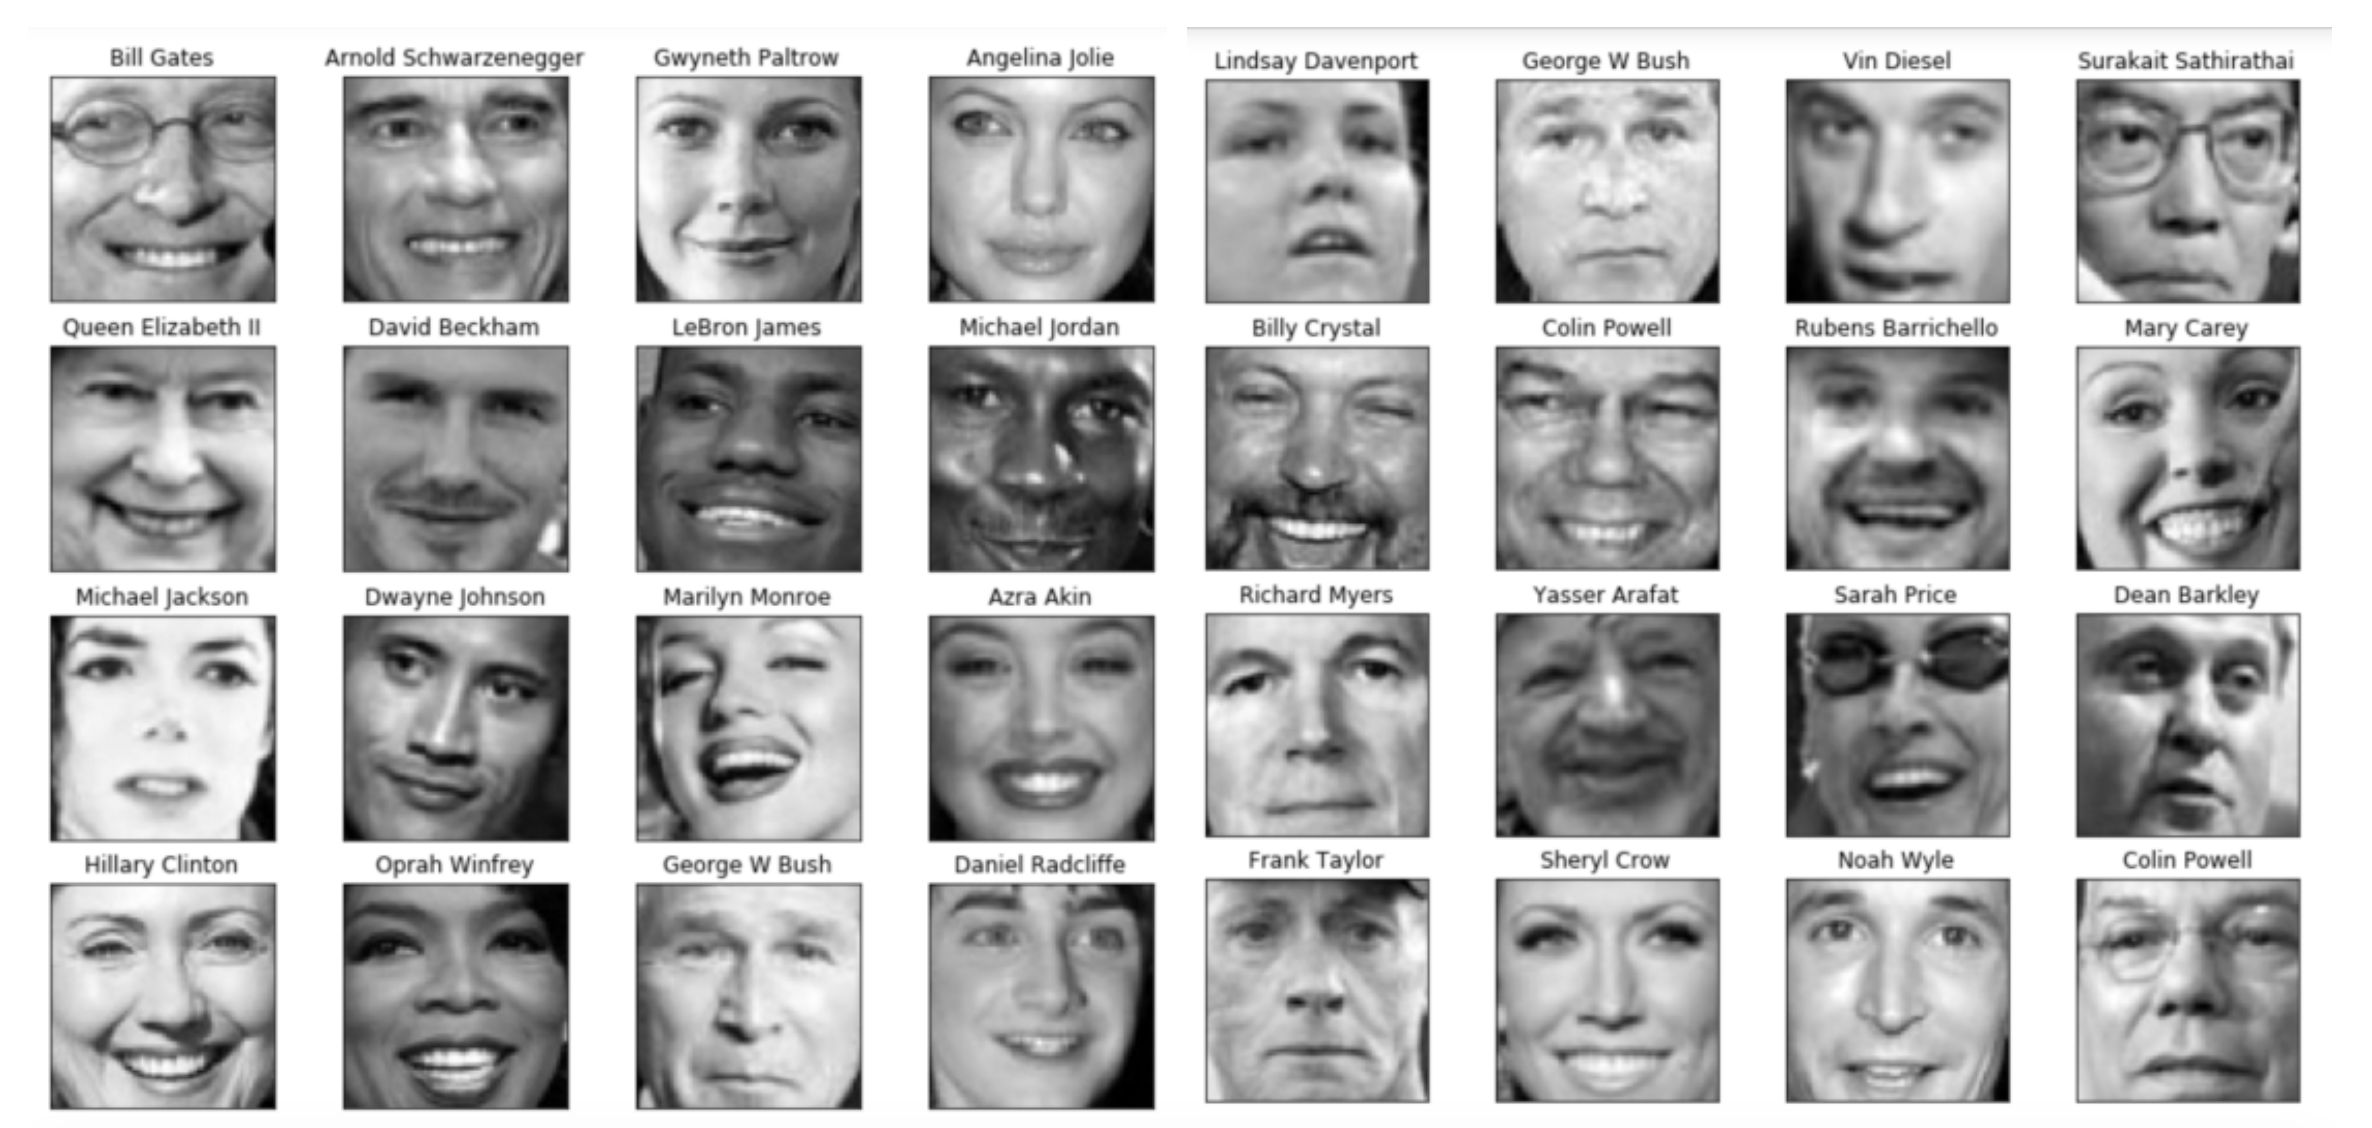
\includegraphics[width=0.8\textwidth]{1000Face} 
\end{center}


\subsection{Task of face recognition}
The task of face recognition is to identify a new image $x$ of a face whether the person is in the dataset $X$ and classify who that is if the person is in $X$. 

A natural idea is to find $i$ such that $$||x-x_i||_2=\min_{1\le j\le N} ||x-x_j||_2$$ or $$i=\arg\min_{1\le j\le N} ||x-x_j||_2.$$ But it doesn't work since different pictures of the same person can have a very large $\ell^2$-distance (between pixels). The solution is projecting the data to a lower dimensional space. 
Then we can find some approximation of the data in a lower dimensional hyperplane for better classification.  To minimize the total distance between the original data and the uncompressed data, we can use PCA for application. 

\subsection{PCA}
Without loss of generality, we assume $\sum x_i=0$. Then we can apply Theorem \ref{theorem:PCA} to find the best projection directions. 

	We use the same notation. Suppose  $\text{dim}\mathbb F = k$, then the optimal projection matrix is $\mathbf{W}=(\mathbf{w}_1,...,\mathbf{w}_k)$, where $\mathbf{w}_i$ is the corresponding eigenvector of the $i$-th big eigenvalue of $\mathbf S=\mathbf X\mathbf X^T$, and $\mathbb F=\text{span}\{\mathbf{w}_1,...,\mathbf{w}_k\}$ ($\mathbf{w}_j^T\mathbf{w}_j=1,\mathbf{w}_i^T\mathbf{w}_j=0, i\neq j$), then the uncompressed data of $\mathbf x_i$ is
	\begin{equation}
		\mathbf{y}_i=\sum_{j=1}^{k}(\mathbf{w}_j^T \mathbf{x}_i)\mathbf{w}_j=\mathbf W\mathbf W^T\mathbf x_i=\mathbf W \tilde{\mathbf x}_i.
	\end{equation}

Moreover, we call the eigenvector of $\mathbf S=\mathbf X\mathbf X^T$, $\mathbf{w}_i$, as EigenFace.  We show the first 16 EigenFaces below. 
\begin{figure}
\begin{center}
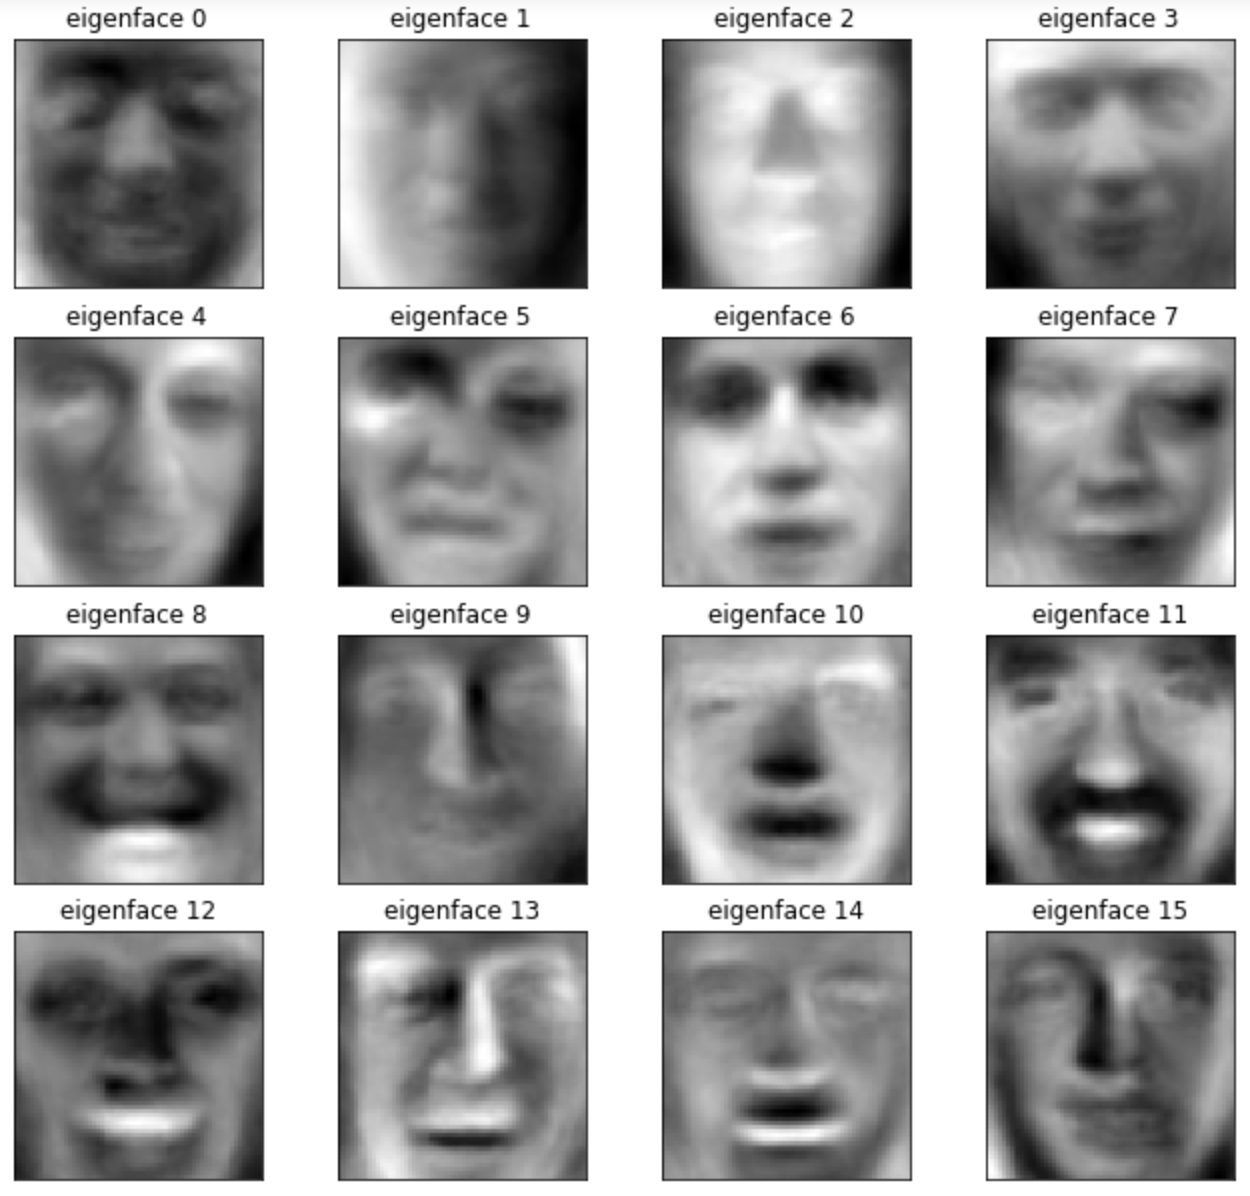
\includegraphics[width=0.5\textwidth]{15EigenFace} 
\caption{Examples of EigenFaces}
\end{center}
\end{figure}

\subsection{Encoding and decoding}
Similarly, we can divide the uncompressed data of $\mathbf x_i$ with two steps, encoding and decoding, where $\tilde{\mathbf x}_i=W^T\mathbf x_i$ is the encoding and $\mathbf{y}_i=\mathbf W \tilde{\mathbf x}_i$ is the decoding part. In detail, the encoding part projects the data to a $k$-dimensional space and we get a lower dimensional coefficient vector $\tilde{\mathbf x}_i=W^T\mathbf x_i$. Thus we can classify faces in this lower dimensional space. Then we can get the the uncompressed data with the decoding part by $\mathbf{y}_i=\mathbf W \tilde{\mathbf x}_i$.

We use the picture of one face data as an example. 
We have an original image: $\mathbf x\in \mathbb{R}^{d}$.
\begin{figure}
\begin{center}
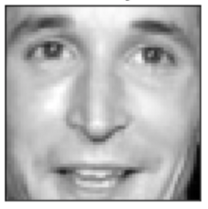
\includegraphics[width=0.4\textwidth]{1000Face-100ori-2} 
\caption{Original image}
\end{center}
\end{figure}
\newpage
After encoding, we get a lower dimensional coefficient vector $\tilde{\mathbf x}=W^T\mathbf x$.
Then after decoding, we get the the uncompressed data
$\mathbf{y}=\mathbf W \tilde{\mathbf x} \in \mathbb{R}^{d}$.
\begin{figure}
\begin{center}
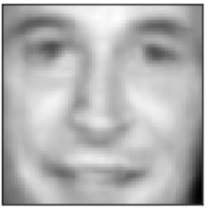
\includegraphics[width=0.4\textwidth]{1000Face-100-2} 
\caption{Uncompressed image}
\end{center}
\end{figure}

\subsection{Classification accuracy}
In the task of face recognition in the dataset of Labeled Faces in the Wild,
PCA extracts features with eigenvectors and achieves 85\% test accuracy in average. 
If we use CNN on this dataset, CNN extracts features with convolutional filters and can achieve 99.85\% test accuracy in average. 



